\documentclass[11pt,twocolumn,letterpaper]{article}

\usepackage{cvpr}
\usepackage{times}
\usepackage{epsfig}
\usepackage{graphicx}
\usepackage{amsmath}
\usepackage{amssymb}
\usepackage{pifont}
\usepackage{subcaption}
\usepackage{float}

\usepackage[breaklinks=true,bookmarks=false]{hyperref}

\cvprfinalcopy

\def\httilde{\mbox{\tt\raisebox{-.5ex}{\symbol{126}}}}

\begin{document}

\title{Feature Extraction from Adversarial Networks for Procedural Terrain Generation}

\author{Jack Serrino\\
{\tt\small jserrino@mit.edu}
\and
Margaret Tian\\
{\tt\small mtian@mit.edu}
\and
Larry Zhang\\
{\tt\small larryq@mit.edu}
}

\maketitle

\begin{abstract}
    Procedural terrain generation has long been explored in video game creation to automatically generate large amounts of new graphical content. Typical methods involve the use of handcrafted, terrain-specific algorithms. We explore the use of a deep convolutional generative adversarial model (DCGAN) to dynamically create realistic terrain maps. Additionally, we introduce a novel method for feature extraction that can be used to specify and modify geographical features of generated terrain.\\
\end{abstract}

\begin{figure*}[ht]
    \centering
    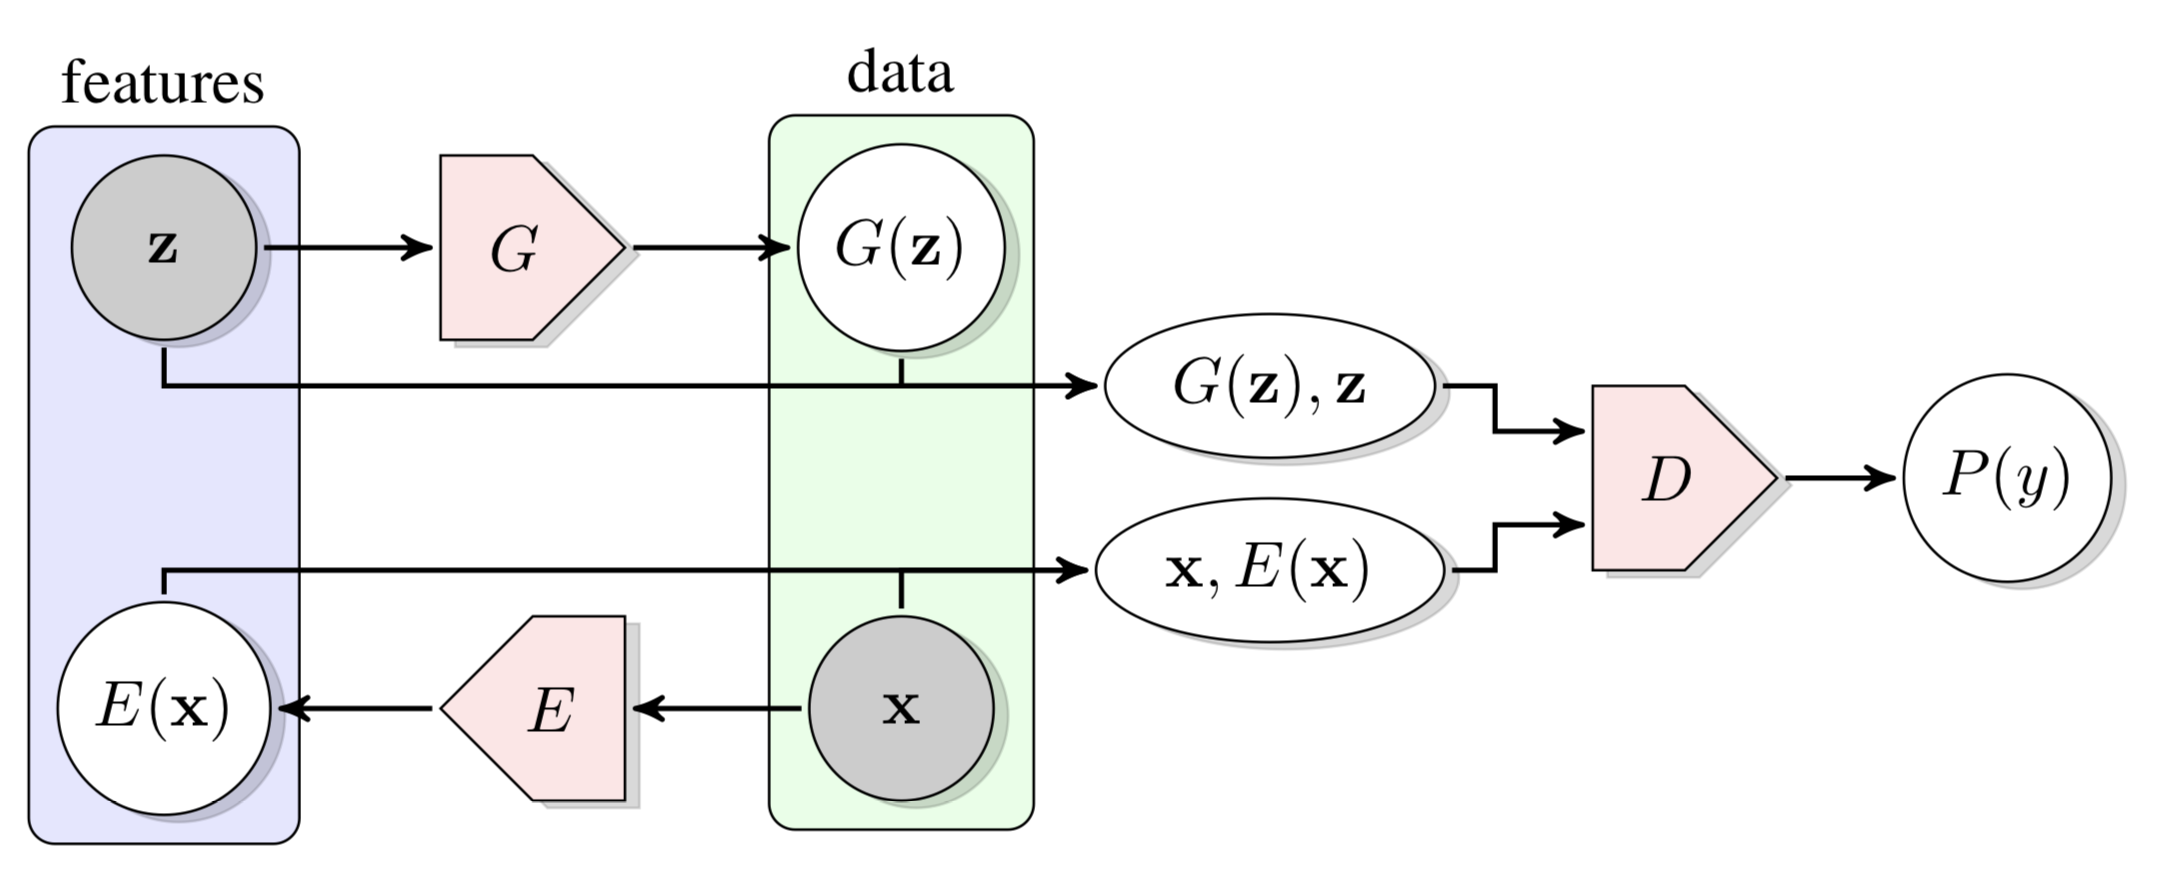
\includegraphics[width=0.9\linewidth]{imgs/bigan.png}
    \caption{Overview of BiGAN architecture from~\cite{bigan}. Note that both the inputs and outputs of the generator and encoder are passed as input to the discriminator.}
  \label{fig:bigan}
\end{figure*}

\section{Introduction}
Procedural generation is the automatic, algorithmic creation of data. It is particularly useful in the context of computer graphics where it can be used to generate textures and 3D models. Many popular open-world video games, such as Minecraft, use procedural generation to create vast, realistic maps at a low cost~\cite{proc-gan}. Current algorithms mimic real-life terrain using things like Perlin noise~\cite{perlin}, but these algorithms lack the control to specify terrain features. Therefore when specific types of terrain are desired, many images must be generated until a match is found, thereby removing the important aspect of full automation. There also exist more complicated software like L3DT~\cite{l3dt}, which do allow the user to control terrain features, (e.g. mountains, lakes, valleys). However, these programs are custom-designed and therefore are not generalizable to unsupported terrain features.

Generative adversarial networks (GANs) have been shown to be powerful frameworks for learning generative models on arbitrarily complex data distributions~\cite{goodfellow}. A GAN is composed of two components: 1) a generator that creates samples that mimic real inputs and 2) a discriminator that distinguishes between the real and generated data. When trained on images, GANs have been shown to produce remarkably realistic results. More recently, deep convolutional GANs (DCGANs) have been proposed as an effective way to model images, since they are able to capture both low-level to high-level image features using convolutional neural architectures. This gives DCGANs more spatial flexibility in generating and discriminating 2D images~\cite{facebook}.

By using the learned weights of the generator, it is possible to control the features in generated images. Since generators take in ``noise'' vectors as input, modifying these vectors allow us to change the contents of the output images. If we can learn which noise vectors correspond to certain features, we can combine the vectors of features we want in order to produce a custom image. In fact, previous work using GANs for procedural terrain generation~\cite{proc-gan} noted that this ability to add, remove, or specify geographical features would be an important next step.

In this paper, we harness the unsupervised learning abilities of DCGANs for procedural terrain generation. Additionally, we introduce a novel method that extracts features from the latent vector space of the generator and performs feature vector arithmetic to customize and modify any terrain image. This allows us to specify the geographical features we would like to see in the output, such as a lake or other body of water.


\section{Contributions}

In order to generate terrain with specifiable geography, we must first learn the latent vector representations of the various types of geography. We do this by extracting features from the vector space of a GAN generator.

Currently, there are two primary methods for extracting features from the latent vector space of a GAN generator. The first is an exhaustive ``guess-and-check'' approach employed in~\cite{facebook}. This feed-forward method simply generates multiple images and selects the corresponding input vectors that are associated with desired outputs. However, this method is difficult to perform precisely due to the high dimensionality of the latent vectors. As a result, it is also extremely unscalable, since a large volume of images must be generated in order to obtain enough samples representative of the target feature.

The second approach is a bidirectional GAN (BiGAN) architecture described in~\cite{bigan}. In addition to the traditional generator and discriminator models, BiGANs have a third encoder model that learns the inverse of the generator. This encoder is a convolutional network that maps inputs in the image space to representations in the latent vector space (Figure~\ref{fig:bigan}), and is trained alongside the generator and discriminator. While this architecture is promising, it requires large amounts of computing power in order to handle the added overhead of the encoder model. Additionally, due to increased number of model weights, the method exacerbates the training stability problem that standard GANs face~\cite{stability}.

Thus, in our paper, we introduce a novel method of feature extraction that learns the latent vector space representation of target images without adding complexity to the GAN architecture. Our approach uses back-propagation to estimate the the nearest noise vector that will generate a given image. While it is not as effective as directly learning the encoder (since we need to perform back-propagation for each target image), it is much more straightforward and easier to train, and is more efficient at learning latent features than blindly guessing and checking. Implementation details are described in Section~\ref{sec:feat-approach}.

In addition to our new feature extraction method, we also explore some use cases of knowing these latent features. By manipulating the vector representations of features, we are directly able to specify characteristics of the output geographical image. Examples are illustrated in Section~\ref{sec:results}.

\begin{figure*}[ht]
    \centering
    \begin{subfigure}[b]{0.24\linewidth}
        \includegraphics[width=\linewidth]{imgs/real1.jpeg}
    \end{subfigure}
    \begin{subfigure}[b]{0.24\linewidth}
        \includegraphics[width=\linewidth]{imgs/real2.jpeg}
    \end{subfigure}
    \begin{subfigure}[b]{0.24\linewidth}
        \includegraphics[width=\linewidth]{imgs/real3.jpeg}
    \end{subfigure}
    \begin{subfigure}[b]{0.24\linewidth}
        \includegraphics[width=\linewidth]{imgs/real_api.jpeg}
    \end{subfigure}
        \caption{Example map tiles shrunk down to $64 \times 64$ pixels. Notice the tile on the right has an ``API KEY REQUIRED'' watermark.}
        \label{fig:tiles}
\end{figure*}

\subsection{Individual Contributions}
All three team members tested different GAN architectures to arrive at the final architecture described in this report. Margaret and Larry focused on preprocessing and handling data, while Jack worked on developing the feature extractor. This report was written collaboratively as a group.

\section{Data}
Our data consists of 20,000 colored map tiles downloaded from the OpenStreetMap Tile database, which can be found at \url{http://wiki.openstreetmap.org/wiki/Tiles}. The map tiles were taken from 100 major cities and surrounding areas from around the world and were captured at a zoom level of 13, which equates to approximately 19 meters per pixel. Examples of our input images can be seen in Figure~\ref{fig:tiles}. This zoom level allowed for enough variation in the geographical features of each tile, without being too close that features of tiles would not be generalizable (Figure~\ref{fig:zoom} illustrates three different zoom levels: 10, 13, and 15). As seen in Figure~\ref{fig:tiles}, some of the map tiles included an ``API KEY REQUIRED'' watermark. We discuss the effects of this watermark on our generator in Section~\ref{sec:results}.

  \begin{figure}[H]
    \centering
        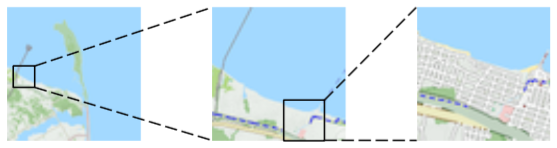
\includegraphics[width=\linewidth]{imgs/zoom.png}
        \caption{Example map tiles at zoom level 10, 13, and 15 (left to right).}
        \label{fig:zoom}
\end{figure}

Due to computational constraints, we preprocess the images by shrinking the original $256 \times 256$ pixel images to $64 \times 64$ pixels using bilinear interpolation. We do not perform color normalization between channels, since the colors of pixels in map images is vital in distinguishing different geographical features (e.g. water vs parks). However, we do normalize image pixel values in all three channels between -1 and 1. We choose to keep map tiles with the ``API KEY REQUIRED'' watermark because the watermark can serve as an easily identifiable ``feature'' of certain images. This way, we can easily test our feature extractor, and subsequently add or remove the watermark from generated map images.

While we added functionality for augmenting our input images (specifically rotation, translation, and mirroring), we did not perform any data augmentation in this iteration of our results.

\begin{figure*}[ht]
  \centering
    \begin{minipage}{.495\linewidth}
    \centering
        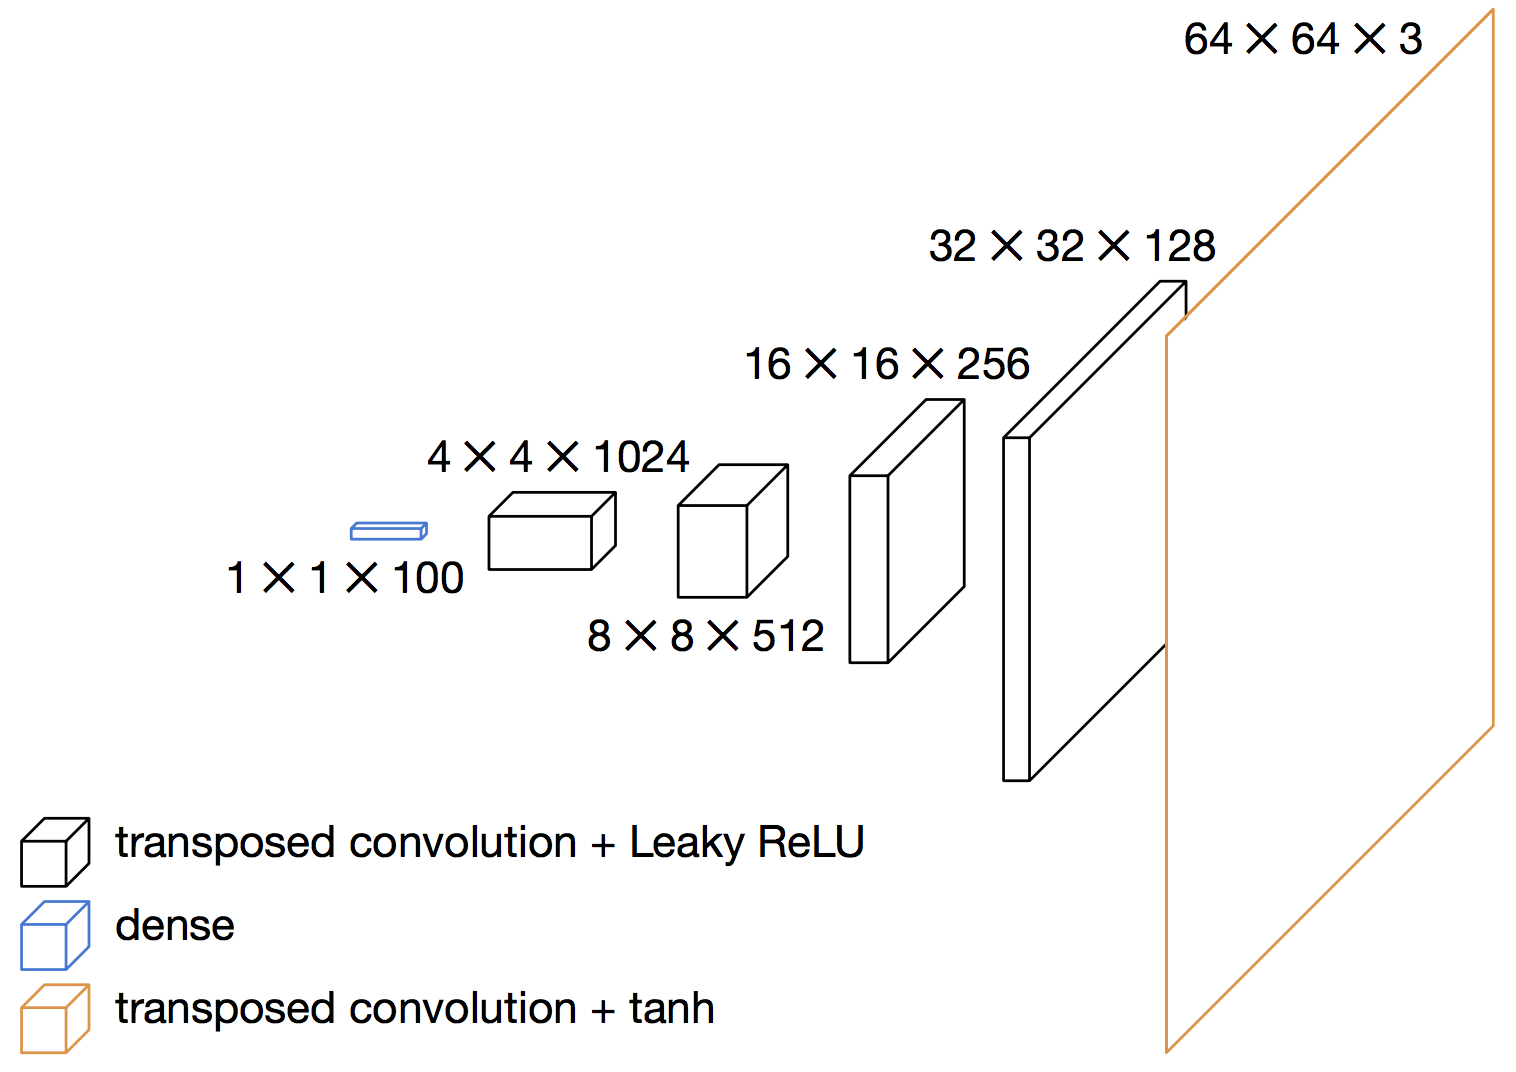
\includegraphics[width=\linewidth]{imgs/generator.png}
        \caption{Generator architecture.}
        \label{fig:gen}
    \end{minipage}
    \quad
    \begin{minipage}{.45\linewidth}
        \centering
        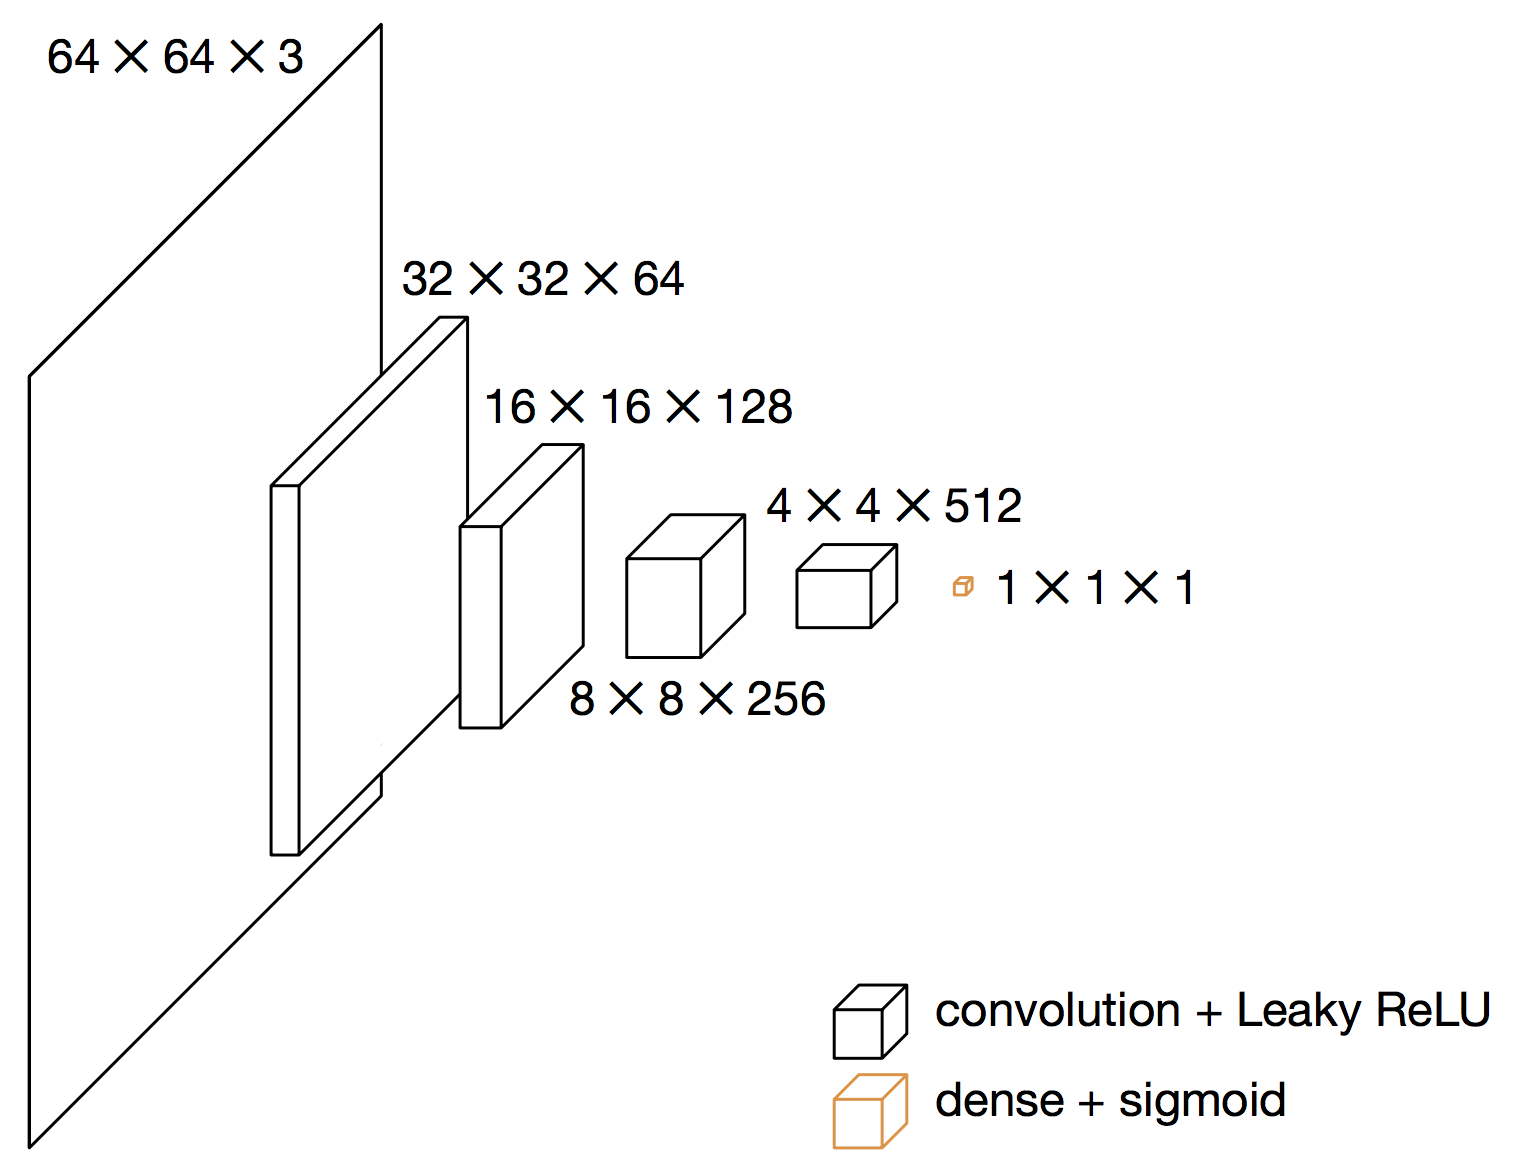
\includegraphics[width=\linewidth]{imgs/discriminator.png}
        \caption{Discriminator architecture.}
        \label{fig:discrim}
    \end{minipage}
\end{figure*}

\section{Approach}

We based our GAN architecture off Facebook's DCGAN~\cite{facebook}. Due to our computational constraints, we chose a relatively simple DCGAN architecture that was sufficient for our purposes. More complex and effective DCGAN architectures exist, and we would hope to explore them in future work. Our implementation is written using the Keras framework~\cite{keras}.

\subsection{GAN Architecture}
Our generator $G$ (Figure~\ref{fig:gen}) takes as input a 100 dimensional noise vector $z$ with mean 0 and standard deviation 1. This vector is then passed through 4 transposed convolutional layers each with Leaky ReLu activation functions. A final $64 \times 64 \times 3$ transposed convolutional layer with $tanh$ activation is used to output a $64 \times 64$ pixel colored image $G(z)$. $tanh$ activation is used since the pixels of the input images are normalized to a range of -1 to 1. To visualize generated image tiles, the normalized pixel outputs for each channel are rescaled to a range of 0 to 255 to produce a standard RGB image.

Our discriminator $D$ (Figure~\ref{fig:discrim}) takes in a normalized $64 \times 64$ 3-channel image $x$ and passes it through 4 convolutional layers each with Leaky ReLu activation functions. Batch normalization layers are also added between convolutional and activation layers. The output layer uses sigmoid activation to predict a probability that the input image is real (i.e. not generated by the generator).

All convolutional and transposed convolutional layers in our GAN use $5 \times 5$ filters with stride 2. Using stride 2 helps us up-sample or down-sample, eliminating the need for pooling and up-sampling layers.


\subsection{Feature extraction} \label{sec:feat-approach}
Given the trained generator of our GAN, we want our extractor to output the closest 100-dimensional feature vector $z$ that will generate an approximation of the given image $x$. We call the learned $z$ the feature representation of $x$. In order to do so, we initialize a guess $z^{(0)}$ as random noise with mean 0 and standard deviation 1. Then we pass this guess as input to the generator to produce an image $G(z^{(0)})$. We calculate the squared error loss of this generated image and the given image $x$:
$$\frac{1}{2} (G(z) - x)^2$$ 
We use standard back-propagation methods to update $z^{(t)}$ with respect to this loss. Note that we do not modify our generator weights during these iterative updates.

Unlike~\cite{bigan} this feature extractor does not learn the inverse of $G$. We must run our feature extraction algorithm for every new image $x$ in order to approximate the corresponding feature representation $v$. However, our method has two main benefits. First, it does not add additional complexity to our GAN architecture. Baseline GAN models are already difficult to train since finding optimal hyperparameters for stable training is hard. Adding additional components thus increases the amount of computing required as well as fine tuning needed for successful training. Our method, although less general than the encoder model implemented in BiGANs, will similarly produce accurate feature representations of images.

Second, our approach at feature extraction is significantly more efficient than blind generation approaches. These ``guess and check'' methods iterate over extremely large quantities of feature vectors and pick from the generated outputs the best image that represents the targeted feature. On the other hand, our feature extractor directly learns the feature representation of the desired target image. Though our back-propagated extraction still takes computation time, it is much more effective than the conventional feed-forward approach.

\section{Results}\label{sec:results}

\begin{figure*}[ht]
    \centering
    \begin{subfigure}[b]{0.24\linewidth}
        \includegraphics[width=\linewidth]{imgs/gen_api1.jpeg}
    \end{subfigure}
    \begin{subfigure}[b]{0.24\linewidth}
        \includegraphics[width=\linewidth]{imgs/gen_api2.jpeg}
    \end{subfigure}
    \begin{subfigure}[b]{0.24\linewidth}
        \includegraphics[width=\linewidth]{imgs/gen_api3.jpeg}
    \end{subfigure}
    \begin{subfigure}[b]{0.24\linewidth}
        \includegraphics[width=\linewidth]{imgs/gen_api4.jpeg}
    \end{subfigure}
        \caption{Examples of generated maps with watermark.}
        \label{fig:generated_api}
\end{figure*}

  \begin{figure*}[ht]
    \centering
    \begin{subfigure}[b]{0.24\linewidth}
        \includegraphics[width=\linewidth]{imgs/gen1.jpeg}
    \end{subfigure}
    \begin{subfigure}[b]{0.24\linewidth}
        \includegraphics[width=\linewidth]{imgs/gen2.jpeg}
    \end{subfigure}
    \begin{subfigure}[b]{0.24\linewidth}
        \includegraphics[width=\linewidth]{imgs/gen3.jpeg}
    \end{subfigure}
    \begin{subfigure}[b]{0.24\linewidth}
        \includegraphics[width=\linewidth]{imgs/gen4.jpeg}
    \end{subfigure}
        \caption{Examples of generated maps without watermark.}
        \label{fig:generated}
\end{figure*}

\subsection{Training}
Training the GAN proved to be difficult. We faced the stability issues that GANs are known for. At early iterations of training, we often found that the generator would produce all-black or white-noise images and the discriminator would therefore be able to perfectly distinguished real and generated inputs. This occurred when the generator and discriminator were trained with the same learning rate of 0.0005. This proved problematic, since the discriminator was learning to distinguish generated images faster than the generator was able to produce realistic images. Thus, weight updates to the generator were not able to lower its loss. Decreasing the learning rate of the discriminator allowed the generator more iterations to reduce generator loss and thus prevented the discriminator from converging prematurely.

However, decreasing discriminator loss also affected later iterations of training, in which we found that the generator was able to always output images that would perfectly fool the discriminator. Finding the correct balance between learning rates to ensure stable training proved to be difficult. Instead, we took a scheduling approach that would repeatedly train the generator until its loss was below a certain ``loss threshold'' before switching and training the discriminator. This method ensured that the generator's loss decreased and simultaneously prevented overfitting.

\subsection{GAN Results}
We trained our GAN for $>$ 25,000 iterations with initial learning rates of 0.0005 after implementing the stability fixes mentioned above. Due to the limit of computing power available to us, our generated images were very noisy. While many macro-level features such as general terrain color and shape were learned, finer details like streets and sharp boundaries were not able to be generated.

As mentioned previously, some of our input map tiles included a watermark containing the words ``API KEY REQUIRED.'' Our generator quickly and successfully learned that generating images with this watermark would decrease its loss. Some examples of generated images with and without the watermark can be seen in Figure~\ref{fig:generated_api} and Figure~\ref{fig:generated}.

  \begin{figure}[ht]
    \centering
    \begin{subfigure}[b]{0.35\linewidth}
    \centering
        \includegraphics[width=\linewidth]{imgs/badcity1.jpeg}
    \end{subfigure}
    \begin{subfigure}[b]{0.35\linewidth}
    \centering
        \includegraphics[width=\linewidth]{imgs/badcity2.jpeg}
    \end{subfigure}    
        \caption{Example generated city tiles.}
        \label{fig:badcity}
\end{figure}

Overall, we see a few general problems with our generator:

\begin{itemize}
\item It is very bad at generating roads and other city-related straight lines 
(Figure~\ref{fig:badcity}). 
This is likely affected by the shrinking step in our preprocessing, since the smaller $64 \times 64$ pixel input images end up with roads that are only a few pixels wide. Additionally, this adds an inherent ``fuzziness'' to sharply defined edges. However, the generator does correctly associate pink, purple, and yellow colors in city areas, which are used to depict roads and buildings in the original inputs. 

\item Water created by our generator contain slight amounts of noise rather than being a uniform blue. However, to the human eye, these patches are still clearly distinguishable as being bodies of water. With better generator filters, we would expect this noise to smooth out and disappear.
\item The generator is particularly good at producing forested and mountainous terrain, since these areas are inherently more random, unlike organized city layouts.
\item The generator is also good at creating maps with mixed terrain (e.g. water and land, city and forest, etc.). We hypothesize that this is due to our filters being less spatially aware, so a terrain type generated in the upper part of the image may be ``forgotten'' when generating the bottom part of the image.
\end{itemize}

In general, many of the problems we see can be attributed to a simple architecture and insufficient computing power. However, our novel methods of feature extraction and image modification still show promising results, as discussed below.

\subsection{Feature Extraction}
To predict the feature vector $v$ for a given image $x$, we perform 200 iterations of back-propagation on an initial random guess. An example of the reconstructed image $G(v)$ using this learned feature vector is shown in Figure~\ref{fig:feature}. From the figure, we see that the generated output has a significant amount of noise, and does not fully capture the details of the original input image. This is very likely a direct result of the poor quality of our GAN and the inability of our generator to accurately produce details and sharp edges. Additionally, it is expected for details to be lost when down-sampling from the image space to the feature vector space. However, the overall shape and position of land and bodies of water is correct, indicating that our feature vector is still reasonably representative in capturing high-level features. It also suggests that a more powerful generator may be able to capture finer details from the input image, and therefore more accurately reconstruct the desired input image.

\begin{figure}[H]
    \centering
        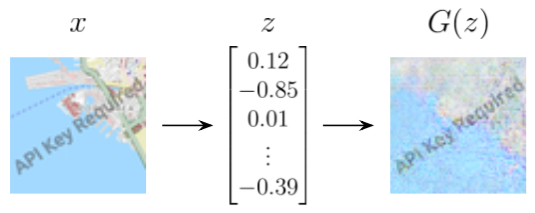
\includegraphics[width=\linewidth]{imgs/feature.png}
        \caption{Example of feature extraction and image reconstruction.}
        \label{fig:feature}
\end{figure}

It is interesting to note that in order to get good feature extraction results, we used an abnormally high learning rate of 100. When the learning rate was too small ($<$ 10) or too large ($>$ 1000), the extractor loss did not improve and no learning occurred. Intuitively, the learning rate needs to be high because large updates in the higher-dimensional image layers are needed in order to translate into noticeable incremental changes in the low-dimensional feature layer.

We also note that the ``API Key Required'' watermark is one of the features that is more accurately preserved in the reconstruction. This validates that the feature learning is capable of extracting relevant information from the input image.

\subsection{Specifiable Feature Generation}

\begin{figure*}[ht]
    \centering
    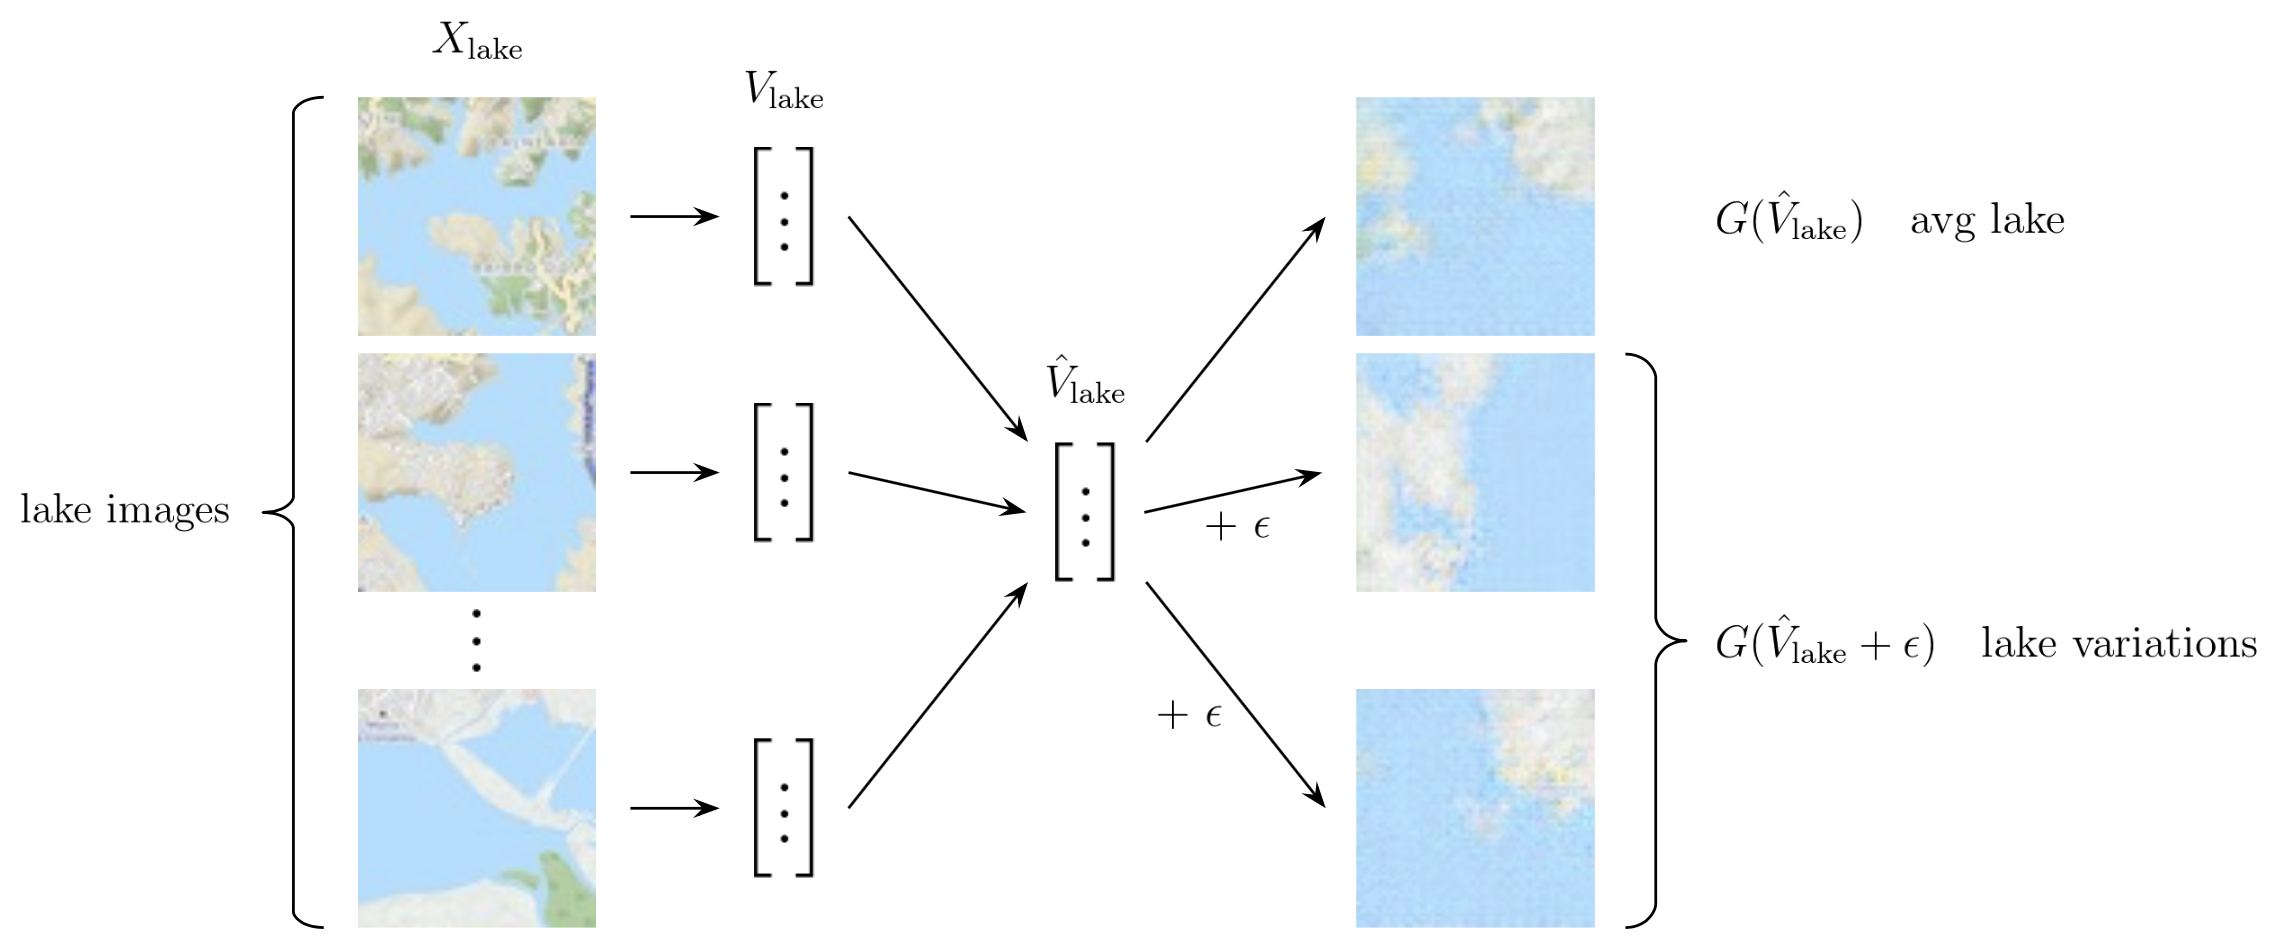
\includegraphics[width=0.95\linewidth]{imgs/lake.png}
    \caption{An illustration of the process behind specifiable feature generation of maps with lakes.}
  \label{fig:lake}
\end{figure*}

Due to the limitations of our GAN and the capabilities of our feature extractor from the previous section, we focus on generating images with specified high-level features, such as bodies of water. Figure~\ref{fig:lake} illustrates this process. First, we sample a subset of images representative of the feature we would like to generate, in this case lakes. We extract the feature vector representation of each of these images and average the feature vectors to obtain an average lake vector $\hat{V}_{\text{lake}}$. Then, we can add random Gaussian noise to this lake vector and feed it through our generator to produce variations of terrain tiles that all contain lakes.

Note that the land masses in the output tiles lose a lot of the specificity present in the input tiles. This is both a byproduct of our generator's performance as well as information loss in feature extraction. However, the content of a lake/land border is still preserved and clearly captured by the average lake vector, thus indicating that our feature extraction method is capable of producing image tiles with specific features.

\subsection{Adding and Removing Features}

\begin{figure*}[ht]
    \centering
    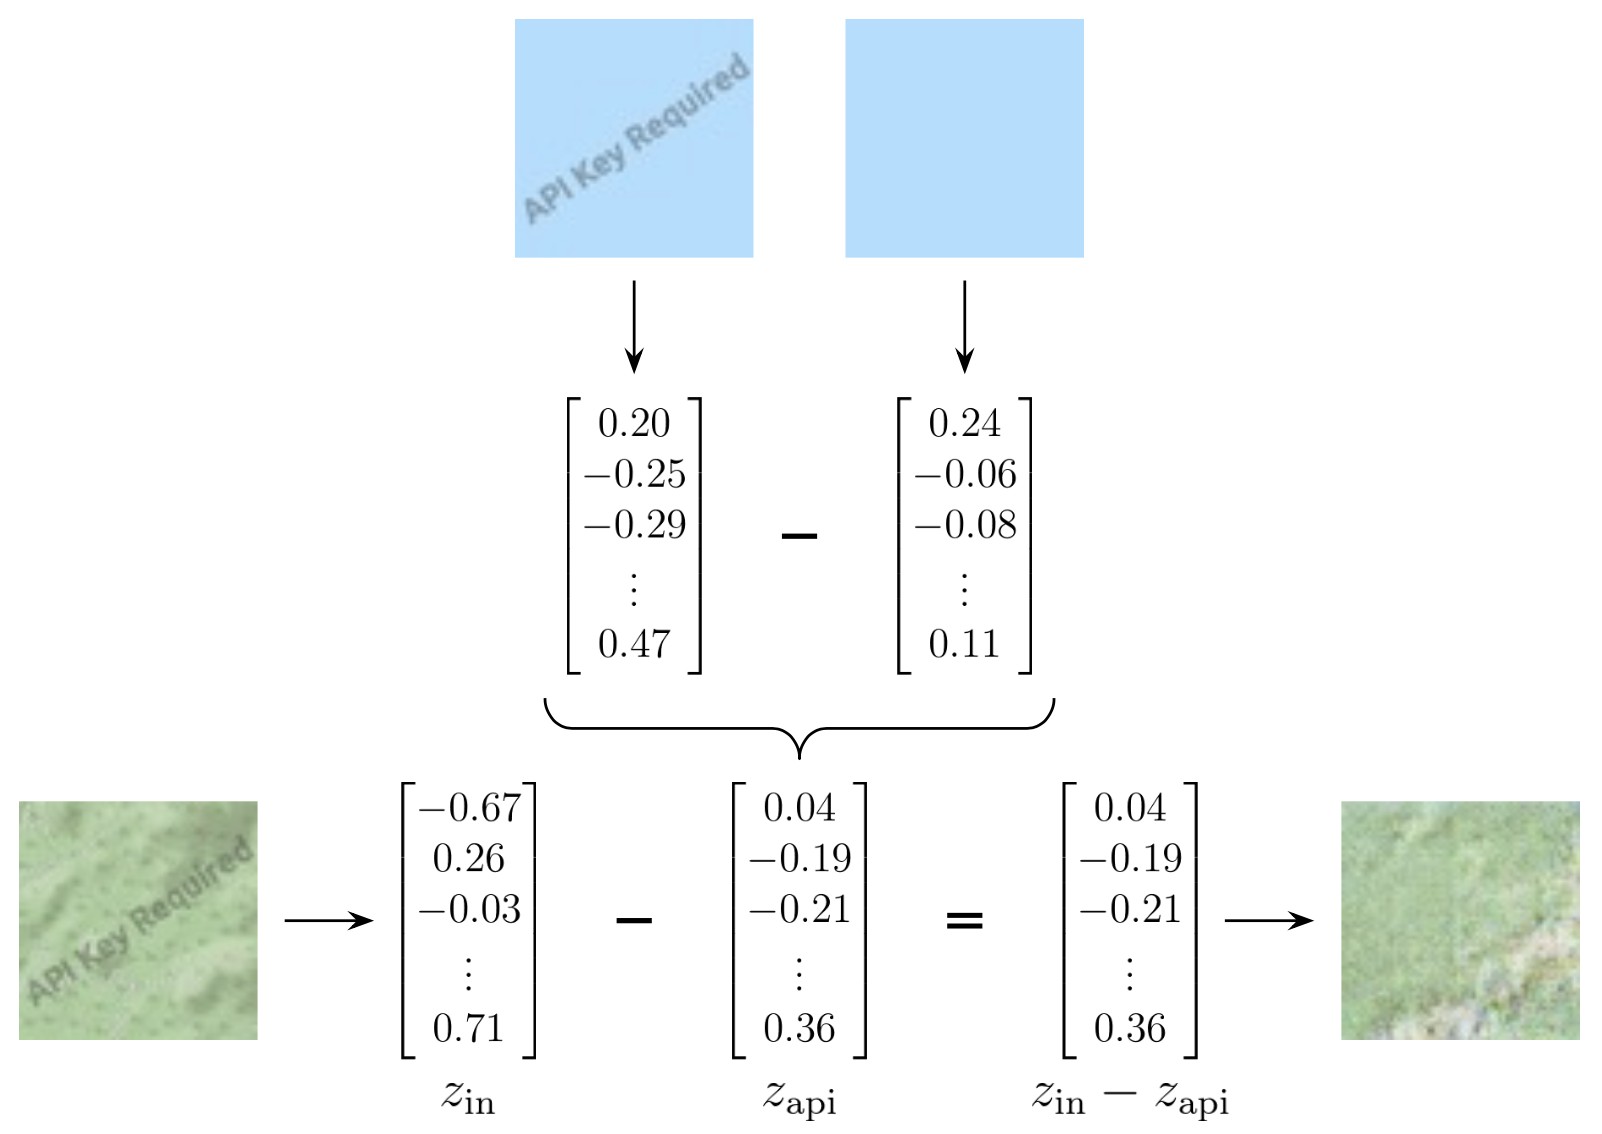
\includegraphics[width=0.75\linewidth]{imgs/api.png}
    \caption{Removal of watermark feature in input image.}
  \label{fig:api}
\end{figure*}

Since our extractor learns feature representations of terrain tiles, it is now much easier to perform vector arithmetic using image feature vectors to add or remove certain elements from existing images. As seen in the previous section, we can easily remove a lake from an image containing both land and water by simply subtracting a lake vector from the feature representation of the image.

We demonstrate this by removing the ``API KEY REQUIRED'' watermark feature from an image, as outlined in Figure~\ref{fig:api}. To get a clear vector representation of the watermark, we take the difference between all-water images with and without the watermark. This then generates $v_{\text{api}}$, the feature vector that encodes the API watermark. Then, by extracting the feature representation of an input image with the watermark, and subtracting $v_{\text{api}}$, we are able to generate a version of the original input without the watermark.

Note that the output image is not a perfect replica of the input. Many of the details are lost and there is some added noise. This is primarily due to the performance of our generator, along with information loss in feature extraction.


\section{Conclusion}
Our work harnesses the generative power of DCGANs to model terrain maps. We introduce a simple, novel method of extracting a feature representation of any terrain image by performing back-propagation on our generator. With these representations, we are able to custom generate maps with specifiable features (e.g. lakes, forests, roads, etc.) and add or remove features on any existing map image. Overall, while this procedure is very straightforward, it still proves to be effective without adding much additional overhead to the already complex GAN architecture.

\subsection{Future Work}
Areas of future work include:
\begin{itemize}
\item Implementing a more complex GAN architecture and performing more training iterations. As mentioned previously, the results from our generator were markedly impacted by our lack of computation power. With more training, we would expect to see clearer images and better results for feature extraction, generation, and modification.
\item Using larger image sizes to retain detailed city features, like sharper roads.
\item Further experimentation with modifying more complicated features (e.g. removing a lake or adding mountainous texture).
\end{itemize}
  

{\small
\bibliographystyle{ieee}
\bibliography{bib}
}

\end{document}
